\Opensolutionfile{ans}[ans/ansCD2D1-5]
\section{Khảo sát sự biến thiên và vẽ đồ thị hàm số}
\subsection{Kiến thức sách giáo khoa cần cần nắm}
\subsubsection{Khảo sát một số hàm đa thức và phân thức}
a) Hàm số bậc 3: $y=ax^3+bx^2+cx+d$ \, $(a\neq 0)$\\
	\renewcommand{\arraystretch}{1} %Thay đổi độ rộng các dòng
\begin{tabular}{|m{2.8cm}|m{4cm}|m{4cm}|}
\hline
\textbf{Trường hợp}	& $$a>0$$	& $$a<0$$\\
	\hline
{$y'=0$ có 2 nghiệm phân biệt ($b^2-3ac>0$)}	& 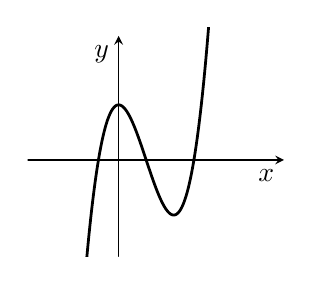
\begin{tikzpicture}[line cap=round,line join=round,>=stealth,x=.5cm,y=.5cm,scale=0.7]
\clip(-3.3,-3.5) rectangle (6.2,4.8);
\draw[->] (-3.3,0)--(6,0) node[below left]{$x$};
\draw[->] (0,-3.5)--(0,4.5) node[below left]{$y$};
\draw[line width=1pt,color=black,smooth,samples=200,domain=-3.3:6] plot(\x,{(\x)^(3.0)-3.0*(\x)^(2.0)+2.0});
\end{tikzpicture} 	& 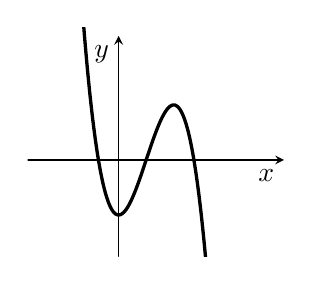
\begin{tikzpicture}[line cap=round,line join=round,>=stealth,x=.5cm,y=.5cm,scale=0.7]
\clip(-3.3,-3.5) rectangle (6.2,4.8);
\draw[->] (-3.3,0)--(6,0) node[below left]{$x$};
\draw[->] (0,-3.5)--(0,4.5) node[below left]{$y$};
\draw[line width=1.2pt,color=black,smooth,samples=100,domain=-3.3:6] plot(\x,{-1*(\x)^(3.0)+3.0*(\x)^(2.0)-2.0});
\end{tikzpicture}\\
	\hline
	%-------------------
 $y'=0$ có nghiệm kép hoặc vô nghiệm ($b^2-3ac\leq 0$)	& 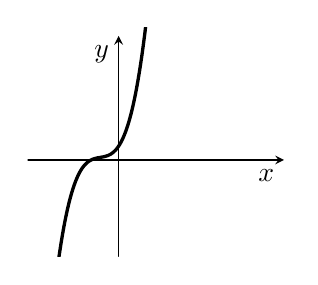
\begin{tikzpicture}[line cap=round,line join=round,>=stealth,x=.5cm,y=.5cm,scale=0.7]
\clip(-3.3,-3.5) rectangle (6.2,4.8);
\draw[->] (-3.3,0)--(6,0) node[below left]{$x$};
\draw[->] (0,-3.5)--(0,4.5) node[below left]{$y$};
\draw[line width=1.2pt,color=black,smooth,samples=100,domain=-3.3:6] plot(\x,{(\x)^(3.0)+2.0*(\x)^(2.0)+1.5*(\x)+0.5});
\end{tikzpicture}	& 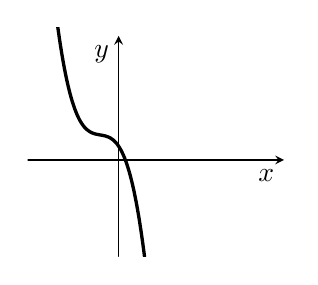
\begin{tikzpicture}[line cap=round,line join=round,>=stealth,x=.5cm,y=.5cm,scale=0.7]
\clip(-3.3,-3.5) rectangle (6.2,4.8);
\draw[->] (-3.3,0)--(6,0) node[below left]{$x$};
\draw[->] (0,-3.5)--(0,4.5) node[below left]{$y$};
\draw[line width=1.2pt,color=black,smooth,samples=100,domain=-3.3:6] plot(\x,{0-(\x)^(3.0)-2.0*(\x)^(2.0)-1.5*(\x)+0.5});
\end{tikzpicture}\\
	
\hline
\end{tabular} 

b) Hàm số trùng phương $y=ax^4+bx^2+c$ \, $(a\neq 0)$.\\

	\begin{tabular}{|m{2.8cm}|m{4cm}|m{4cm}|}
	\hline 
\textbf{Trường hợp} & $$a>0$$ & $$a<0$$ \\ 
	\hline 
	Phương trình $y'=0$ có $3$ nghiệm phân biệt ($a.b<0$) & 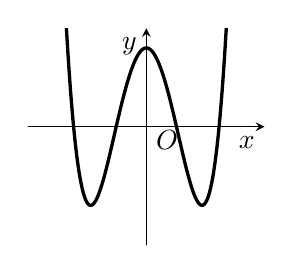
\begin{tikzpicture}[line cap=round,line join=round,>=stealth,scale=0.5]
	\draw[->,color=black] (-3,0) -- (3,0) node[below left]{$x$};
	\draw[->,color=black] (0,-3) -- (0.,2.5)  node[below left]{$y$};
	\draw[color=black] (0pt,-10pt) node[right] {$O$};
	\clip(-3,-3) rectangle (3,2.5);
	\draw[line width=1.2pt,color=black,smooth,samples=200,domain=-3:3] plot(\x,{(\x)^(4.0)-4.0*(\x)^(2.0)+2.0});
	\end{tikzpicture} & 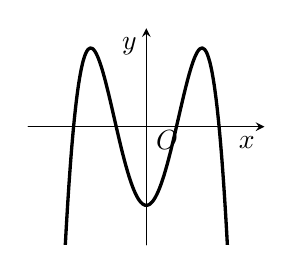
\begin{tikzpicture}[line cap=round,line join=round,>=stealth,scale=0.5]
		\draw[->,color=black] (-3,0) -- (3,0) node[below left]{$x$};
	\draw[->,color=black] (0,-3) -- (0.,2.5) node[below left]{$y$};
	\draw[color=black] (0pt,-10pt) node[right] {$O$};
	\clip(-3,-3) rectangle (3,2.5);
	\draw[line width=1.2pt,color=black,smooth,samples=100,domain=-3.0:3.0] plot(\x,{0-(\x)^(4.0)+4.0*(\x)^(2.0)-2.0});
	\end{tikzpicture} \\ 
	\hline 
Phương trình $y'=0$ có $1$ nghiệm ($a.b\geq 0$) &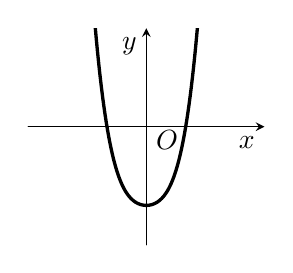
\begin{tikzpicture}[line cap=round,line join=round,>=stealth,scale=0.5]
	\draw[->,color=black] (-3,0) -- (3,0) node[below left]{$x$};
\draw[->,color=black] (0,-3) -- (0.,2.5) node[below left]{$y$};
\draw[color=black] (0pt,-10pt) node[right] {$O$};
\clip(-3,-3) rectangle (3,2.5);
	\draw[line width=1.2pt,color=black,smooth,samples=100,domain=-3.0:3.0] plot(\x,{(\x)^(4.0)+(\x)^(2.0)-2.0});
	\end{tikzpicture} & 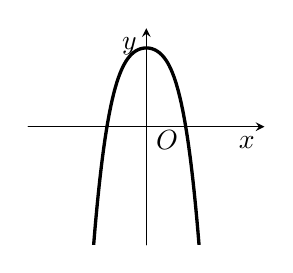
\begin{tikzpicture}[line cap=round,line join=round,>=stealth,scale=0.5]
	\draw[->,color=black] (-3,0) -- (3,0) node[below left]{$x$};
\draw[->,color=black] (0,-3) -- (0.,2.5) node[below left]{$y$};
\draw[color=black] (0pt,-10pt) node[right] {$O$};
\clip(-3,-3) rectangle (3,2.5);
	\draw[line width=1.2pt,color=black,smooth,samples=100,domain=-3.0:3.0] plot(\x,{0-(\x)^(4.0)-(\x)^(2.0)+2.0});
	\end{tikzpicture} \\ 
	\hline 
\end{tabular} 


c) Hàm phân thức $y=\dfrac{ax+b}{cx+d},\left(ab-bc\neq 0\right)$.
\begin{center}
	\begin{tabular}{|m{4cm}|m{4cm}|}
	\hline 
	\begin{center}
		Khi $ad-bc>0$
	\end{center} & \begin{center}
	Khi $ad-bc<0$
\end{center} \\ 
	\hline 
	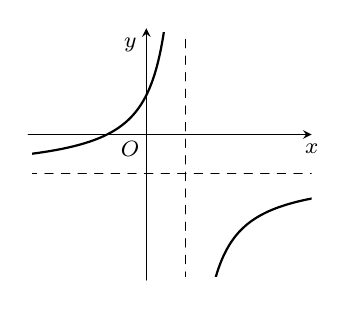
\begin{tikzpicture}[>=stealth, font=\footnotesize, line join=round, line cap=round,scale=0.5]
\def\a{1} \def\b{1} \def\c{-1} \def\d{1}
\draw[->] (-3,0)--(4.2,0) node [below]{$x$};
\draw[->] (0,-3.7)--(0,2.7) node [below left]{$y$};
\node at (0,0) [below left=-1pt]{$O$};
\clip (-2.9,-3.6) rectangle (4.2,2.6);
\draw[thick,smooth,samples=300,domain=-3:(-\d/\c-0.1)] plot(\x,{(\a*(\x)+\b)/(\c*(\x)+\d)});
\draw[thick,smooth,samples=300,domain=(-\d/\c+0.1:4.2)] plot(\x,{(\a*(\x)+\b)/(\c*(\x)+\d)});
\draw[dashed] (-\d/\c,-3.7)--(-\d/\c,2.7);
\draw[dashed] (-3,\a/\c)--(4.2,\a/\c);
\end{tikzpicture} & 	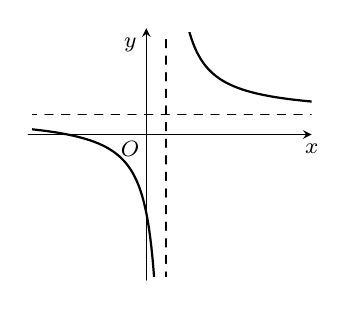
\begin{tikzpicture}[>=stealth, font=\footnotesize, line join=round, line cap=round,scale=0.5]
\def\a{1} \def\b{2} \def\c{2} \def\d{-1}
\draw[->] (-3,0)--(4.2,0) node [below]{$x$};
\draw[->] (0,-3.7)--(0,2.7) node [below left]{$y$};
\node at (0,0) [below left=-1pt]{$O$};
\clip (-2.9,-3.6) rectangle (4.2,2.6);
\draw[thick,smooth,samples=300,domain=-3:(-\d/\c-0.1)] plot(\x,{(\a*(\x)+\b)/(\c*(\x)+\d)});
\draw[thick,smooth,samples=300,domain=(-\d/\c+0.1:4.2)] plot(\x,{(\a*(\x)+\b)/(\c*(\x)+\d)});
\draw[dashed] (-\d/\c,-3.7)--(-\d/\c,2.7);
\draw[dashed] (-3,\a/\c)--(4.2,\a/\c);
%\foreach \x in {-2,-1,1}
%\draw (\x,0.05)node[below]{$\x$}--(\x,-0.05);
%\foreach \y in {-1,1,2}
%\draw (-0.05,\y)node[right]{$\y$}--(0.05,\y);
\end{tikzpicture}\\ 
	\hline 
\end{tabular}
\end{center}
\subsection{Phân loại và phương pháp giải bài tập}
\begin{dang}{Các phép biến đổi đồ thị}
\begin{enumerate}
	\item $f(x) \xrightarrow{{\text{tịnh tiến trái phải }m \text{ đvị}}} f(x+m)$.
	\item $f(x) \xrightarrow{{\text{tịnh tiến lên xuống }m \text{ đvị}}} f(x)+m$.
	\item $f(x) \xrightarrow[{\text{giữ phải, bỏ trái } Oy}]{{\text{đối xứng phải sang trái}}} f(|x|)$.
	\item $f(x) \xrightarrow[{\text{giữ trên }Ox}]{{\text{đối xứng dưới lên trên}}} |f(x)|$.
\end{enumerate}
\end{dang}
\begin{note}
Nếu vừa xuất hiện đối xứng, vừa tịnh tiến thì thực hiện theo quy tắc 
\begin{center}
	 $x$ \textit{ngoài vào,} $y$ \textit{trong ra}.
\end{center}
\end{note}
\subsubsection{Các ví dụ}
\begin{vd}%Ví dụ 1.%[2D1B5-2]
	Từ đồ thị $(C)\colon y=f(x)=x^3-3x+2$ suy ra đồ thị $(C')$: $y=|x|^3-3|x|+2$.\\
	Biến đổi $(C)$:\\
	+ Bỏ phần đồ thị $(C)$ bên trái $Oy$, giữ nguyên $(C)$ bên phải $Oy$.\\
	+ Lấy đối xứng phần đồ thị được giữ lại qua $Oy$. 
\begin{center}
	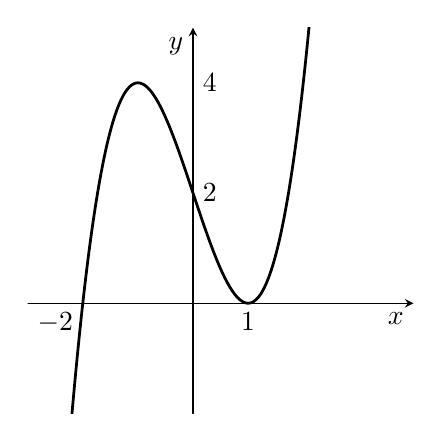
\begin{tikzpicture}[line cap=round,line join=round,>=stealth,scale=0.7]
\clip(-3,-2) rectangle (4,5);
\draw[->] (-3,0)--(4,0) node[below left]{$x$};
\draw[->] (0,-2)--(0,5) node[below left]{$y$};
\draw (-2,0) node[below left] {$-2$};
\draw (1,0) node[below] {$1$};
\draw (0,4) node[right] {$4$} (0,2) node[right] {$2$} ;
\draw[line width=1pt,color=black,smooth,samples=200,domain=-3.3:6] plot(\x,{(\x)^(3.0)-3.0*(\x)+2.0});
\end{tikzpicture}
\begin{tikzpicture}[line cap=round,line join=round,>=stealth,scale=0.5]
\clip(-0.2,-3) rectangle (3.5,4);
\draw[-] (0,2)--(2,2)--(2,2.5)--(3,1.5)--(2,0.5)--(2,1)--(0,1)--(0,2);
\end{tikzpicture}
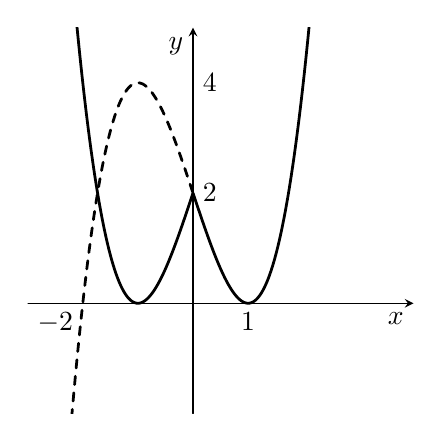
\begin{tikzpicture}[line cap=round,line join=round,>=stealth,scale=0.7]
\clip(-3,-2) rectangle (4,5);
\draw[->] (-3,0)--(4,0) node[below left]{$x$};
\draw[->] (0,-2)--(0,5) node[below left]{$y$};
\draw (-2,0) node[below left] {$-2$};
\draw (1,0) node[below] {$1$};
\draw (0,4) node[right] {$4$} (0,2) node[right] {$2$} ;
\draw[dashed,line width=1pt,color=black,smooth,samples=200,domain=-3.3:0] plot(\x,{(\x)^(3.0)-3.0*(\x)+2.0});
\draw[line width=1pt,color=black,smooth,samples=200,domain=-3.3:0] plot(\x,{-1*(\x)^(3.0)+3.0*(\x)+2.0});
\draw[line width=1pt,color=black,smooth,samples=200,domain=0:6] plot(\x,{(\x)^(3.0)-3.0*(\x)+2.0});
\end{tikzpicture}
\end{center}
%<MyLT>
\end{vd}
\begin{vd}%Ví dụ 1.%[2D1B5-2]
	Từ đồ thị $(C)\colon y=f(x)=x^3-3x+2$ suy ra đồ thị hàm số $y=\left|x^3-3x+2\right|$.\\
	Biến đổi $(C)$:\\
	+ Bỏ phần đồ thị $(C)$ dưới $Ox$, giữ nguyên $(C)$ phía trên $Ox$.\\
	+ Lấy đối xứng phần đồ thị bị bỏ qua $Ox$ 
\begin{center}
	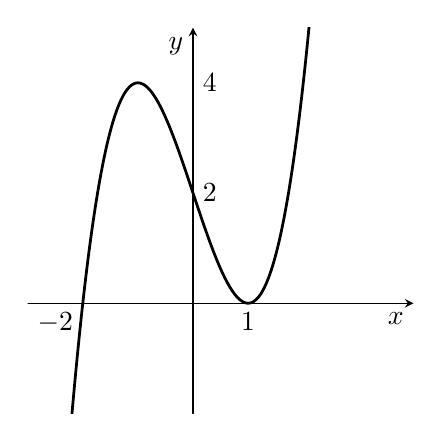
\begin{tikzpicture}[line cap=round,line join=round,>=stealth,scale=0.7]
	\clip(-3,-2) rectangle (4,5);
	\draw[->] (-3,0)--(4,0) node[below left]{$x$};
	\draw[->] (0,-2)--(0,5) node[below left]{$y$};
	\draw (-2,0) node[below left] {$-2$};
	\draw (1,0) node[below] {$1$};
	\draw (0,4) node[right] {$4$} (0,2) node[right] {$2$} ;
	\draw[line width=1pt,color=black,smooth,samples=200,domain=-3.3:6] plot(\x,{(\x)^(3.0)-3.0*(\x)+2.0});
	\end{tikzpicture}
	\begin{tikzpicture}[line cap=round,line join=round,>=stealth,scale=0.5]
	\clip(-0.2,-3) rectangle (3.5,4);
	\draw[-] (0,2)--(2,2)--(2,2.5)--(3,1.5)--(2,0.5)--(2,1)--(0,1)--(0,2);
	\end{tikzpicture}
	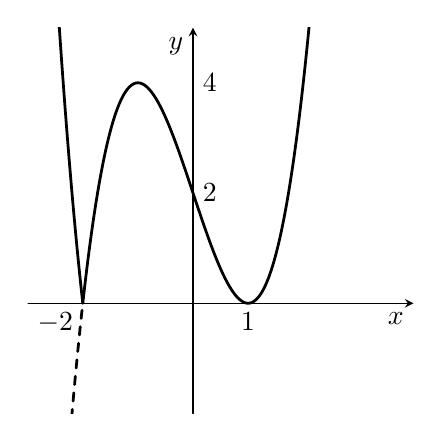
\begin{tikzpicture}[line cap=round,line join=round,>=stealth,scale=0.7]
	\clip(-3,-2) rectangle (4,5);
	\draw[->] (-3,0)--(4,0) node[below left]{$x$};
	\draw[->] (0,-2)--(0,5) node[below left]{$y$};
	\draw (-2,0) node[below left] {$-2$};
	\draw (1,0) node[below] {$1$};
	\draw (0,4) node[right] {$4$} (0,2) node[right] {$2$} ;
	\draw[line width=1pt,color=black,smooth,samples=200,domain=-2:6] plot(\x,{(\x)^(3.0)-3.0*(\x)+2.0});
	\draw[line width=1pt,color=black,smooth,samples=200,domain=-3.3:-2] plot(\x,{-1*(\x)^(3.0)+3.0*(\x)-2.0});
	\draw[dashed,line width=1pt,color=black,smooth,samples=200,domain=-3.3:-2] plot(\x,{(\x)^(3.0)-3.0*(\x)+2.0});
	\end{tikzpicture}
\end{center}
%<MyLT>
\end{vd}
Chú ý: Với dạng $y=\left|f(|x|)\right|$ ta lần lượt biến đổi 2 đồ thị $y=f(|x|)$ và $y=\left|f(x)\right|$.\\
\begin{vd}%[2D1B5-2]
	Từ đồ thị $(C)\colon y=f(x)=x^3-3x$ suy ra đồ thị $y=\left||x|^3-3|x|\right|$.\\
	Biến đổi $(C)$ để được đồ thị $(C')\colon y=|x|^3-3|x|$.\\
	Biến đổi $(C')\colon y=|x|^3-3|x|$ ta được đồ thị $(C'')$: $y=\left||x|^3-3|x|\right|$ 
\begin{center}
		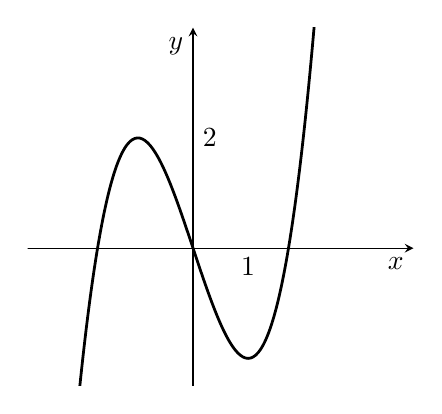
\begin{tikzpicture}[line cap=round,line join=round,>=stealth,scale=0.7]
\clip(-3,-2.5) rectangle (4,4);
\draw[->] (-3,0)--(4,0) node[below left]{$x$};
\draw[->] (0,-2.5)--(0,4) node[below left]{$y$};
\draw (1,0) node[below] {$1$};
\draw (0,2) node[right] {$2$} ;
\draw[line width=1pt,color=black,smooth,samples=200,domain=-3.3:6] plot(\x,{(\x)^(3.0)-3.0*(\x)});
\end{tikzpicture}
\begin{tikzpicture}[line cap=round,line join=round,>=stealth,scale=0.5]
\clip(-0.2,-3) rectangle (3.5,4);
\draw[-] (0,2)--(2,2)--(2,2.5)--(3,1.5)--(2,0.5)--(2,1)--(0,1)--(0,2);
\end{tikzpicture}
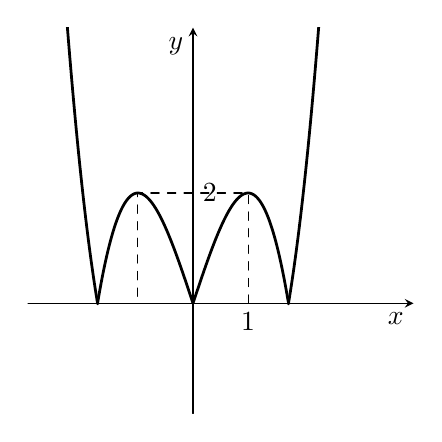
\begin{tikzpicture}[line cap=round,line join=round,>=stealth,scale=0.7]
\clip(-3,-2) rectangle (4,5);
\draw[->] (-3,0)--(4,0) node[below left]{$x$};
\draw[->] (0,-2)--(0,5) node[below left]{$y$};
\draw[dashed](1,0)--(1,2)--(-1,2)--(-1,0);
\draw (1,0) node[below] {$1$};
\draw (0,2) node[right] {$2$} ;
\draw[line width=1pt,color=black,smooth,samples=200,domain=1.73:6] plot(\x,{(\x)^(3.0)-3.0*(\x)});
\draw[line width=1pt,color=black,smooth,samples=200,domain=0:1.73] plot(\x,{-1*(\x)^(3.0)+3.0*(\x)});
\draw[line width=1pt,color=black,smooth,samples=200,domain=-1.73:0] plot(\x,{(\x)^(3.0)-3.0*(\x)});
\draw[line width=1pt,color=black,smooth,samples=200,domain=-3.3:-1.73] plot(\x,{-1*(\x)^(3.0)+3.0*(\x)});
\end{tikzpicture}
\end{center}
%<MyLT>
\end{vd}
\Closesolutionfile{ans}	
